\documentclass[aspectratio=169,10pt]{beamer}

\usepackage[utf8]{inputenc}
\usepackage[T1]{fontenc}
\usepackage{amsmath,amssymb,amsthm}
\usepackage{graphicx}
\usepackage{listings}
\usepackage{xcolor}
\usepackage{tikz}
\usetikzlibrary{positioning,arrows.meta}
\usepackage{algorithm}
\usepackage{algorithmic}
\usepackage{hyperref}
\usepackage{mimic}

\usetheme{Madrid}
\usecolortheme{seahorse}
\setbeamertemplate{navigation symbols}{}
\setbeamertemplate{footline}[frame number]

\lstset{
    language=Python,
    basicstyle=\ttfamily\scriptsize,
    keywordstyle=\color{blue}\bfseries,
    stringstyle=\color{red},
    commentstyle=\color{green!60!black},
    showstringspaces=false,
    breaklines=true,
    breakatwhitespace=true,
    frame=single,
    numbers=left,
    numberstyle=\tiny\color{gray},
    xleftmargin=1em,
    framexleftmargin=1em,
    escapechar=@
}

% Title page information
\title{Reinforcement Learning}
\subtitle{Lecture 9: Actor-Critic Methods}
\author{Taehoon Kim}
\institute{Sogang University MIMIC Lab \\ \url{https://mimic-lab.com}}
\date{Fall Semester 2025}

\begin{document}

% Slide 1: Title
\begin{frame}
\titlepage
\end{frame}

% Slide 2: Today's Agenda
\begin{frame}{Today's Agenda}
\begin{itemize}
    \item Why move beyond vanilla policy gradients
    \item Value baselines, advantage estimation, and GAE
    \item Actor-Critic architectures and vectorised A2C
    \item Entropy regularisation and tuning workflows
    \item Hands-on experiments and integrated A2C run
\end{itemize}
\end{frame}

% Slide 3: Learning Objectives
\begin{frame}{Learning Objectives}
By the end of this lecture, you will:

\textbf{Theory Understanding:}
\begin{itemize}
    \item Explain why Actor-Critic reduces variance vs vanilla policy gradients
    \item Derive n-step and GAE advantage estimators
    \item Analyze bias-variance trade-offs in bootstrapping
\end{itemize}

\textbf{Practical Skills:}
\begin{itemize}
    \item Implement vectorized A2C with proper GAE computation
    \item Configure entropy regularization for exploration
    \item Train scalable agents across multiple environments
    \item Report ablations over entropy coefficient and return horizon
\end{itemize}

\textbf{Prerequisites:} Policy gradients, value functions, PyTorch basics
\end{frame}

% Slide 4: Motivation - The Variance Problem
\begin{frame}{The Variance Problem in Policy Gradients}
\textbf{REINFORCE Algorithm Recap:}
$$\nabla_\theta J(\theta) = \mathbb{E}[\nabla_\theta \log \pi_\theta(a|s) \cdot G_t]$$

\textbf{Problems:}
\begin{itemize}
    \item High variance in gradient estimates
    \item Slow convergence due to noisy updates
    \item Sample inefficiency
\end{itemize}

\textbf{Solution Ideas:}
\begin{itemize}
    \item Use a baseline to reduce variance: $G_t - b(s_t)$
    \item Learn the baseline from data: $b(s_t) = V(s_t)$
    \item Combine policy learning with value learning
\end{itemize}

$\Rightarrow$ \textbf{Actor-Critic Methods}
\end{frame}

% Slide 5: Actor-Critic Concept
\begin{frame}{Actor-Critic: Best of Both Worlds}
\begin{columns}
\begin{column}{0.5\textwidth}
\textbf{Actor (Policy):}
\begin{itemize}
    \item Learns policy $\pi_\theta(a|s)$
    \item Selects actions
    \item Updated via policy gradients
\end{itemize}

\textbf{Critic (Value Function):}
\begin{itemize}
    \item Learns value $V_\phi(s)$
    \item Evaluates actions
    \item Provides baseline for actor
\end{itemize}
\end{column}
\begin{column}{0.5\textwidth}
\begin{center}
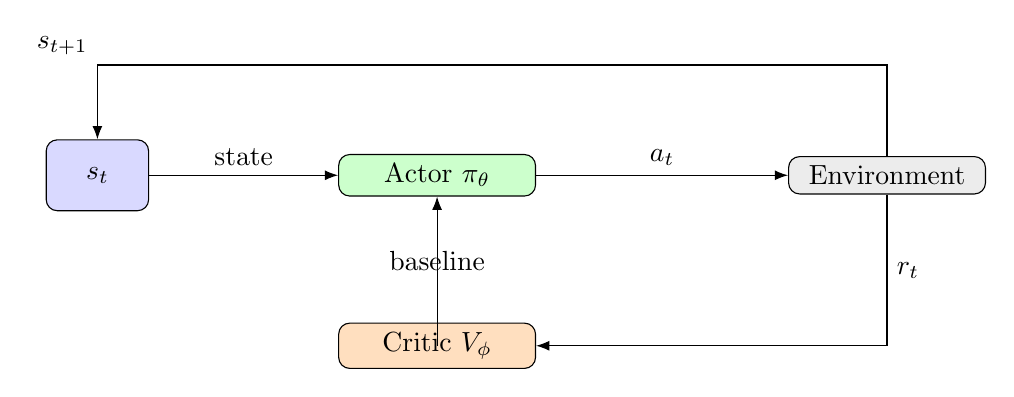
\begin{tikzpicture}[>=Latex]
    \node[draw, rounded corners, fill=blue!15, minimum width=1.3cm, minimum height=0.9cm] (state) {$s_t$};
    \node[draw, rounded corners, fill=green!20, right=2.4cm of state, minimum width=2.5cm] (actor) {Actor $\pi_\theta$};
    \node[draw, rounded corners, fill=orange!25, below=1.6cm of actor, minimum width=2.5cm] (critic) {Critic $V_\phi$};
    \node[draw, rounded corners, fill=gray!15, right=3.2cm of actor, minimum width=2.5cm] (env) {Environment};

    \draw[->] (state) -- node[above] {state} (actor);
    \draw[->] (actor) -- node[above] {$a_t$} (env);
    \draw[->] (env) |- node[pos=0.25, right] {$r_t$} (critic);
    \draw[->] (critic) -| node[pos=0.85, below] {baseline} (actor);
    \draw[->] (env) -- ++(0,1.4) -| node[above left] {$s_{t+1}$} (state);
\end{tikzpicture}
\end{center}
\end{column}
\end{columns}

\textbf{Key Insight:} Critic provides learned baseline, reducing variance while maintaining policy gradient benefits.
\end{frame}

% Slide 6: Mathematical Foundation
\begin{frame}{Mathematical Foundation}
\textbf{Policy Gradient with Baseline:}
$$\nabla_\theta J(\theta) = \mathbb{E}[\nabla_\theta \log \pi_\theta(a|s) \cdot (Q^\pi(s,a) - V^\pi(s))]$$

\textbf{Define Advantage Function:}
$$A^\pi(s,a) = Q^\pi(s,a) - V^\pi(s)$$

\textbf{Advantage Interpretation:}
\begin{itemize}
    \item How much better is action $a$ compared to average?
    \item $A^\pi(s,a) > 0$: action better than average
    \item $A^\pi(s,a) < 0$: action worse than average
    \item $A^\pi(s,a) = 0$: action is average
\end{itemize}

\textbf{Gradient Becomes:}
$$\nabla_\theta J(\theta) = \mathbb{E}[\nabla_\theta \log \pi_\theta(a|s) \cdot A^\pi(s,a)]$$
\end{frame}

% Slide 7: Estimating Advantages
\begin{frame}{Estimating Advantages: The Challenge}
\textbf{Problem:} We don't know true $A^\pi(s,a) = Q^\pi(s,a) - V^\pi(s)$

\textbf{Solution Options:}
\begin{enumerate}
    \item \textbf{Monte Carlo:} $\hat{A}_t = G_t - V(s_t)$
    \begin{itemize}
        \item $G_t = \sum_{k=0}^{\infty} \gamma^k r_{t+k}$
        \item Low bias, high variance
    \end{itemize}
    
    \item \textbf{TD(0):} $\hat{A}_t = r_t + \gamma V(s_{t+1}) - V(s_t)$
    \begin{itemize}
        \item Uses bootstrapping
        \item High bias, low variance
    \end{itemize}
    
    \item \textbf{n-step:} Interpolate between MC and TD
    
    \item \textbf{GAE:} Exponentially weighted average
\end{enumerate}
\end{frame}

% Slide 8: N-Step Returns
\begin{frame}{N-Step Advantage Estimation}
\textbf{N-Step Return:}
$$G_t^{(n)} = \sum_{k=0}^{n-1} \gamma^k r_{t+k} + \gamma^n V(s_{t+n})$$

\textbf{N-Step Advantage:}
$$\hat{A}_t^{(n)} = G_t^{(n)} - V(s_t)$$

\textbf{Special Cases:}
\begin{itemize}
    \item $n=1$: $\hat{A}_t^{(1)} = r_t + \gamma V(s_{t+1}) - V(s_t)$ (TD error)
    \item $n=\infty$: $\hat{A}_t^{(\infty)} = G_t - V(s_t)$ (Monte Carlo)
\end{itemize}

\textbf{Bias-Variance Trade-off:}
\begin{itemize}
    \item Small $n$: Low variance, high bias
    \item Large $n$: High variance, low bias
\end{itemize}
\end{frame}

% Slide 9: Generalized Advantage Estimation (GAE)
\begin{frame}{Generalized Advantage Estimation (GAE)}
\textbf{Key Idea:} Exponentially weighted average of all n-step advantages

\textbf{GAE Formula:}
$$\hat{A}_t^{\text{GAE}(\gamma,\lambda)} = \sum_{\ell=0}^{\infty} (\gamma\lambda)^\ell \delta_{t+\ell}$$

where $\delta_t = r_t + \gamma V(s_{t+1}) - V(s_t)$ is the TD error.

\textbf{Alternative Form:}
$$\hat{A}_t^{\text{GAE}} = (1-\lambda) \sum_{n=1}^{\infty} \lambda^{n-1} \hat{A}_t^{(n)}$$

\textbf{Lambda Parameter:}
\begin{itemize}
    \item $\lambda = 0$: GAE = TD error (low variance, high bias)
    \item $\lambda = 1$: GAE = Monte Carlo (high variance, low bias)
    \item $\lambda \in [0.9, 0.97]$: Common practical range
\end{itemize}
\end{frame}

% Slide 10: GAE Computation
\begin{frame}[fragile]{GAE Computation (Backward Pass)}
\textbf{Efficient Implementation:}

\begin{lstlisting}[language=Python]
def compute_gae(rewards, values, terminated, gamma=0.99, lam=0.95):
    T, N = rewards.shape
    advantages = torch.zeros(T, N)
    last_adv = torch.zeros(N)
    
    for t in reversed(range(T)):
        nonterminal = (not terminated[t]).float()
        next_value = values[t+1] * nonterminal
        
        # TD error
        delta = rewards[t] + gamma * next_value - values[t]
        
        # GAE recursion
        last_adv = delta + gamma * lam * last_adv * nonterminal
        advantages[t] = last_adv
    
    returns = advantages + values[:-1]
    return advantages, returns
\end{lstlisting}

\textbf{Key Points:} Backward computation, terminal state masking, bootstrap handling
\end{frame}

% Slide 11: A2C Algorithm Overview
\begin{frame}{Advantage Actor-Critic (A2C) Algorithm}
\textbf{Synchronous A2C Steps:}
\begin{enumerate}
    \item \textbf{Collect} rollouts from $N$ parallel environments for $T$ steps
    \item \textbf{Compute} advantages using GAE
    \item \textbf{Update} actor using policy gradient with advantages
    \item \textbf{Update} critic using value function regression
    \item \textbf{Repeat}
\end{enumerate}

\textbf{Key Features:}
\begin{itemize}
    \item On-policy learning
    \item Parallel data collection
    \item Shared network architecture (optional)
    \item Entropy regularization for exploration
\end{itemize}

\textbf{vs A3C:} A2C uses synchronous updates vs A3C's asynchronous updates
\end{frame}

% Slide 12: A2C Loss Functions
\begin{frame}{A2C Loss Functions}
\textbf{Policy Loss (Actor):}
$$L_{\text{policy}} = -\mathbb{E}[\log \pi_\theta(a_t|s_t) \cdot \hat{A}_t]$$

\textbf{Value Loss (Critic):}
$$L_{\text{value}} = \frac{1}{2}\mathbb{E}[(G_t - V_\phi(s_t))^2]$$

\textbf{Entropy Loss (Exploration):}
$$L_{\text{entropy}} = -\mathbb{E}[\mathcal{H}(\pi_\theta(\cdot|s_t))]$$

\textbf{Combined Loss:}
$$L_{\text{total}} = L_{\text{policy}} + c_v L_{\text{value}} + \beta L_{\text{entropy}}$$

\textbf{Hyperparameters:}
\begin{itemize}
    \item $c_v \approx 0.5$: Value loss coefficient
    \item $\beta \in [0.001, 0.01]$: Entropy coefficient
\end{itemize}
\end{frame}

% Slide 13: Advantage Normalization
\begin{frame}{Advantage Normalization}
\textbf{Why Normalize?}
\begin{itemize}
    \item Advantages can have different scales across episodes
    \item Normalization improves optimization stability
    \item Standard practice in modern implementations
\end{itemize}

\textbf{Normalization Formula:}
$$\hat{A}_{t,\text{norm}} = \frac{\hat{A}_t - \mu}{\sigma + \epsilon}$$

where:
\begin{itemize}
    \item $\mu = \frac{1}{B}\sum_{i=1}^B \hat{A}_i$ (batch mean)
    \item $\sigma = \sqrt{\frac{1}{B}\sum_{i=1}^B (\hat{A}_i - \mu)^2}$ (batch std)
    \item $\epsilon = 10^{-8}$ (numerical stability)
    \item $B = T \times N$ (batch size)
\end{itemize}

\textbf{Effect:} Zero mean, unit variance advantages within each batch
\end{frame}

% Slide 14: Network Architecture
\begin{frame}{Network Architecture Choices}
\textbf{Shared Trunk Architecture:}
\centering
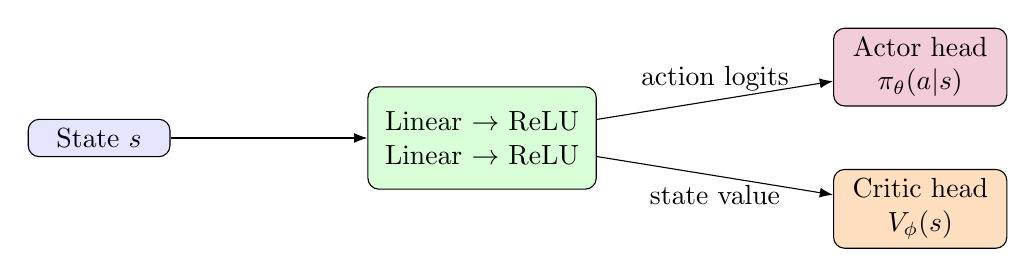
\begin{tikzpicture}[>=Latex, node distance=2cm, every node/.style={align=center}]
    \node[draw, rounded corners, fill=blue!10, minimum width=1.8cm] (input) {State $s$};
    \node[draw, rounded corners, fill=green!15, right=2.5cm of input, minimum width=2.9cm, minimum height=1.3cm] (shared) {Linear $\rightarrow$ ReLU\\Linear $\rightarrow$ ReLU};
    \node[draw, rounded corners, fill=purple!20, right=3cm of shared, yshift=0.9cm, minimum width=2.2cm] (actor) {Actor head\\$\pi_\theta(a|s)$};
    \node[draw, rounded corners, fill=orange!25, right=3cm of shared, yshift=-0.9cm, minimum width=2.2cm] (critic) {Critic head\\$V_\phi(s)$};

    \draw[->] (input) -- node[above] {} (shared);
    \draw[->] (shared) -- node[above] {action logits} (actor);
    \draw[->] (shared) -- node[below] {state value} (critic);
\end{tikzpicture}

\textbf{Separate Networks:}
\begin{itemize}
    \item Independent actor and critic networks
    \item More parameters, potentially better representation
    \item Higher computational cost
\end{itemize}

\textbf{Trade-offs:}
\begin{itemize}
    \item Shared: Parameter efficiency, faster training
    \item Separate: Representational flexibility, avoid interference
\end{itemize}
\end{frame}

% Slide 15: Entropy Regularization Deep Dive
\begin{frame}{Entropy Regularization: Encouraging Exploration}
\textbf{Shannon Entropy:}
$$\mathcal{H}(\pi) = -\sum_a \pi(a|s) \log \pi(a|s)$$

\textbf{Properties:}
\begin{itemize}
    \item Maximum for uniform distribution: $\log|\mathcal{A}|$
    \item Minimum (0) for deterministic policy
    \item Encourages balanced action selection
\end{itemize}

\textbf{Effect of Entropy Coefficient $\beta$:}
\begin{itemize}
    \item $\beta = 0$: No exploration bonus, fast convergence to local optimum
    \item $\beta$ small: Balanced exploration-exploitation
    \item $\beta$ large: Too much exploration, slow convergence
\end{itemize}

\textbf{Scheduling:} Often decrease $\beta$ over training (exploration $\to$ exploitation)
\end{frame}

% Slide 16: Handling Episode Boundaries
\begin{frame}[fragile]{Handling Terminated vs Truncated Episodes}
\textbf{Gymnasium Convention:}
\begin{itemize}
    \item \texttt{terminated}: Episode ended naturally (game over)
    \item \texttt{truncated}: Episode ended artificially (time limit)
\end{itemize}

\textbf{Bootstrapping Rules:}
\begin{itemize}
    \item If \texttt{terminated}: Next value = 0 (episode truly ended)
    \item If \texttt{truncated}: Bootstrap from $V(s_{next})$ (episode continues)
\end{itemize}

\textbf{Implementation:}
\begin{lstlisting}[language=Python]
# Mask for bootstrapping
next_value = values[t+1] * (not terminated[t]).float()
delta = rewards[t] + gamma * next_value - values[t]
\end{lstlisting}

\textbf{Why Important:} Incorrect handling leads to biased value estimates
\end{frame}

% Slide 17: Vectorized Environments
\begin{frame}[fragile]{Vectorized Environments for Efficiency}
\textbf{Concept:} Run multiple environment instances in parallel

\textbf{Benefits:}
\begin{itemize}
    \item Higher throughput (environment steps per second)
    \item Better GPU utilization
    \item More diverse experience per update
    \item Reduced correlation in collected data
\end{itemize}

\textbf{Implementation:}
\begin{lstlisting}[language=Python]
from gymnasium.vector import SyncVectorEnv

# Create N parallel environments
envs = SyncVectorEnv([make_env() for _ in range(N)])

# Step all environments simultaneously  
obs, rewards, terminated, truncated, infos = envs.step(actions)
# obs.shape = [N, obs_dim]
# rewards.shape = [N]
\end{lstlisting}

\textbf{Typical Setup:} N=16, T=128 $\rightarrow$ 2048 samples per update
\end{frame}

% Slide 18: Bias-Variance Trade-off Analysis
\begin{frame}{Bias-Variance Trade-off in Advantage Estimation}
\begin{center}
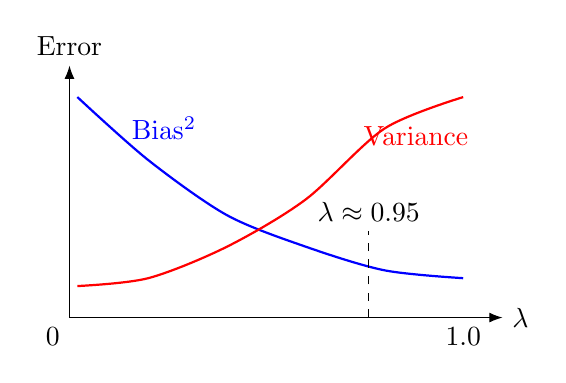
\begin{tikzpicture}[scale=1.0, >=Latex]
    \draw[->] (0,0) -- (5.5,0) node[right] {$\lambda$};
    \draw[->] (0,0) -- (0,3.2) node[above] {Error};
    \draw (0,0) node[below left] {0};
    \draw (5,0) node[below] {1.0};

    % Bias curve (decreasing)
    \draw[thick, blue] plot[smooth] coordinates {(0.1,2.8) (1,2.0) (2,1.3) (3,0.9) (4,0.6) (5,0.5)};
    % Variance curve (increasing)
    \draw[thick, red] plot[smooth] coordinates {(0.1,0.4) (1,0.5) (2,0.9) (3,1.5) (4,2.4) (5,2.8)};
    % Annotate sweet spot
    \draw[dashed] (3.8,0) -- (3.8,1.1);
    \node[above] at (3.8,1.1) {$\lambda \approx 0.95$};
    \node[blue] at (1.2,2.4) {Bias$^2$};
    \node[red] at (4.4,2.3) {Variance};
\end{tikzpicture}
\end{center}

\textbf{Key Insights:}
\begin{itemize}
    \item $\lambda=0$ (TD): Low variance, high bias
    \item $\lambda=1$ (MC): High variance, low bias  
    \item $\lambda \in [0.9, 0.97]$: Sweet spot for most tasks
    \item Total error = bias$^2$ + variance
\end{itemize}

\textbf{Empirical Guidelines:}
\begin{itemize}
    \item Start with $\lambda=0.95$
    \item Increase for long episodes or sparse rewards
    \item Decrease for short episodes or dense rewards
\end{itemize}
\end{frame}

% Slide 19: A2C vs Other Methods
\begin{frame}{A2C vs Other Methods}
\begin{center}
\begin{tabular}{|l|c|c|c|c|}
\hline
\textbf{Method} & \textbf{Sample Eff.} & \textbf{Stability} & \textbf{Complexity} & \textbf{Parallelization} \\
\hline
REINFORCE & Low & Low & Low & Easy \\
\hline
A2C & Medium & Medium & Medium & Easy \\
\hline
PPO & Medium-High & High & Medium & Easy \\
\hline
DQN & High & Medium & Medium & Hard \\
\hline
SAC & High & High & High & Hard \\
\hline
\end{tabular}
\end{center}

\textbf{A2C Advantages:}
\begin{itemize}
    \item Simpler than PPO, more stable than REINFORCE  
    \item Good baseline for policy gradient methods
    \item Excellent for educational purposes
    \item Fast iteration during development
\end{itemize}

\textbf{A2C Limitations:}
\begin{itemize}
    \item Can be unstable with large learning rates
    \item Less sample efficient than off-policy methods
\end{itemize}
\end{frame}

% Slide 20: Gradient Clipping
\begin{frame}[fragile]{Gradient Clipping in A2C}
\textbf{Why Clip Gradients?}
\begin{itemize}
    \item Policy gradients can be noisy and large
    \item Large updates can destabilize learning
    \item Common in all policy gradient methods
\end{itemize}

\textbf{Gradient Norm Clipping:}
$$g \leftarrow \frac{g}{\max(1, \|g\|_2 / \text{max\_grad\_norm})}$$

\textbf{Implementation:}
\begin{lstlisting}[language=Python]
# Compute gradients
loss.backward()

# Clip gradients
torch.nn.utils.clip_grad_norm_(
    model.parameters(), 
    max_norm=0.5
)

# Update parameters
optimizer.step()
\end{lstlisting}

\textbf{Typical Values:} max\_grad\_norm $\in [0.1, 1.0]$, commonly 0.5
\end{frame}

% Slide 21: Theory Summary
\begin{frame}{Theory Summary: Key Concepts}
\textbf{Core Ideas:}
\begin{itemize}
    \item \textbf{Actor-Critic:} Combine policy gradients with value functions
    \item \textbf{Advantage:} $A(s,a) = Q(s,a) - V(s)$ reduces variance
    \item \textbf{GAE:} Elegant interpolation between TD and MC estimates
    \item \textbf{Entropy:} Regularization prevents premature convergence
\end{itemize}

\textbf{Mathematical Foundation:}
\begin{align}
\nabla_\theta J(\theta) &= \mathbb{E}[\nabla_\theta \log \pi_\theta(a|s) \cdot A(s,a)] \\
\hat{A}_t^{\text{GAE}} &= \sum_{\ell=0}^{\infty} (\gamma\lambda)^\ell \delta_{t+\ell} \\
L &= L_{\text{policy}} + c_v L_{\text{value}} - \beta \mathcal{H}(\pi)
\end{align}

\textbf{Ready for Implementation!}
\end{frame}

\section{Hands-on Experiments}

% Slide 22: Implementation Roadmap
\begin{frame}{Implementation Roadmap}
\textbf{Experiment Sequence (9 experiments):}
\begin{enumerate}
    \item \texttt{exp01\_setup.py} -- environment + vector env verification
    \item \texttt{exp02\_value\_functions.py} -- Monte Carlo value estimates
    \item \texttt{exp03\_policy\_gradient\_review.py} -- gradient sanity check
    \item \texttt{exp04\_actor\_critic\_architecture.py} -- shared trunk network
    \item \texttt{exp05\_advantage\_methods.py} -- n-step vs GAE comparison
    \item \texttt{exp06\_gae\_implementation.py} -- effect of different $\lambda$
    \item \texttt{exp07\_vectorized\_a2c.py} -- synchronous A2C with 4 envs
    \item \texttt{exp08\_entropy\_analysis.py} -- entropy coefficient sweep
    \item \texttt{exp09\_integrated\_a2c.py} -- integrated A2C smoke test
\end{enumerate}

\textbf{Learning Progression:} Building blocks $\rightarrow$ Integration $\rightarrow$ Optimization
\end{frame}

% Slide 23: Standard Code Header
\begin{frame}[fragile]{Standard Code Header}
\textbf{PyTorch 2.x Best Practices:}

\begin{lstlisting}[language=Python]
import os, random, numpy as np, torch
import torch.nn as nn
import torch.optim as optim
from torch.distributions import Categorical
import gymnasium as gym

def setup_seed(seed=42):
    random.seed(seed)
    np.random.seed(seed) 
    torch.manual_seed(seed)
    if torch.cuda.is_available():
        torch.cuda.manual_seed_all(seed)

# Proper device selection (CUDA > MPS > CPU)
device = torch.device(
    'cuda' if torch.cuda.is_available()
    else 'mps' if hasattr(torch.backends, 'mps') and torch.backends.mps.is_available()
    else 'cpu'
)
setup_seed(42)
\end{lstlisting}
\end{frame}

% Slide 24: Experiment 1 - Setup Verification
\begin{frame}[fragile]{Experiment 1: Setup Verification}
\textbf{File:} \texttt{exp01\_setup.py}

\textbf{What it checks}
\begin{itemize}
    \item Package versions (Python, PyTorch, Gymnasium)
    \item Preferred compute device (CUDA/MPS/CPU)
    \item Reproducible seeding (tensor statistics under seed 2024)
    \item Vector environment reset/step sanity check
\end{itemize}

\begin{lstlisting}[language=Python]
from gymnasium.vector import SyncVectorEnv

env = SyncVectorEnv([lambda: gym.make("CartPole-v1")
                     for _ in range(4)])
obs, _ = env.reset(seed=2024)
print(obs.shape)  # (4, 4)
actions = env.action_space.sample()
obs, reward, terminated, truncated, _ = env.step(actions)
\end{lstlisting}

\textbf{Latest run (seed 2024)}
\begin{itemize}
    \item Versions -- Python \textbf{3.12.11}, PyTorch \textbf{2.7.1}, Gymnasium \textbf{1.2.0}
    \item Device detected: \textbf{cpu} (MPS unavailable on host)
    \item Vector obs shape: \textbf{(4, 4)}; reward sample \textbf{[1, 1, 1, 1]}
    \item Snapshot saved to \texttt{figures/lecture09\_exp01\_env\_snapshot.json}
\end{itemize}
\end{frame}
% Slide 25: Experiment 2 - Value Functions
\begin{frame}[fragile]{Experiment 2: Value Function Basics}
\textbf{File:} \texttt{exp02\_value\_functions.py}

\textbf{What we measured}
\begin{itemize}
    \item 25 random-policy episodes on CartPole-v1
    \item Monte Carlo estimate of $V(s_t)$ for each time step
    \item Average episode return: \textbf{19.7 $\pm$ 10.9}
    \item Value at $t=0$: \textbf{19.70}, decaying to \textbf{16.40} by $t=4$
\end{itemize}

\begin{center}
\includegraphics[width=0.8\linewidth]{figures/value_estimate_random_policy.png}
\vspace{0.25em}
{\scriptsize Monte Carlo $V(s_t)$ profile for a random CartPole policy.}
\end{center}

\textbf{Takeaway:} returns decay quickly even for short horizons -- a prime motivation for online actor-critic updates instead of full-episode Monte Carlo targets.
\end{frame}
% Slide 26: Experiment 3 - Policy Gradients
\begin{frame}[fragile]{Experiment 3: Policy Gradient Review}
\textbf{File:} \texttt{exp03\_policy\_gradient\_review.py}

\begin{itemize}
    \item Tiny two-action policy with parameter $\theta=0.3$
    \item Compare analytical, autograd, and finite-difference gradients
    \item Autograd: \textbf{0.425557}; Finite difference: \textbf{0.425547}; Closed form: \textbf{0.425557}
    \item Absolute error between autograd and FD: \textbf{$1.0\times10^{-5}$}
\end{itemize}

\begin{lstlisting}[language=Python]
logits = policy(obs)
dist = Categorical(logits=logits.squeeze(0))
log_prob = dist.log_prob(torch.tensor(0))
autograd_grad = torch.autograd.grad(log_prob, policy.theta)[0]
# Finite difference, closed form comparisons follow...
\end{lstlisting}

\textbf{Takeaway:} our actor gradient implementation matches theory to numerical precision.
\end{frame}
% Slide 27: Experiment 4 - Actor-Critic Architecture
\begin{frame}[fragile]{Experiment 4: Actor-Critic Architecture}
\textbf{File:} \texttt{exp04\_actor\_critic\_architecture.py}

\begin{itemize}
    \item Shared trunk: Linear-ReLU-Linear-ReLU
    \item Actor head: linear layer producing action logits
    \item Critic head: linear layer producing scalar $V(s)$
    \item Total parameters: \textbf{17,539} (actor head \textbf{258}, critic head \textbf{129})
    \item Sample logits: $[0.255, -0.069]$; value prediction: \textbf{-0.1787}
\end{itemize}

\begin{lstlisting}[language=Python]
model = ActorCritic(obs_dim=4, act_dim=2)
logits, value = model(torch.randn(5, 4))
print(logits.shape, value.shape)  # torch.Size([5, 2]), torch.Size([5])
\end{lstlisting}

\textbf{Outcome:} reusable module powering all subsequent A2C experiments.
\end{frame}
% Slide 28: Experiment 5 - Advantage Methods
\begin{frame}[fragile]{Experiment 5: Advantage Computation Methods}
\textbf{File:} \texttt{exp05\_advantage\_methods.py}

\begin{itemize}
    \item Synthetic rollout of length 20 (random rewards, decaying baseline)
    \item Compare 1-step, 3-step, Monte Carlo, and GAE ($\lambda = 0.95$)
    \item Monte Carlo mean advantage: \textbf{+10.31} (std \textbf{5.00})
    \item GAE $\lambda = 0.95$ mean advantage: \textbf{+7.67} (std \textbf{3.01})
    \item 1-step TD mean advantage: \textbf{+0.996} (std \textbf{0.246})
\end{itemize}

\begin{lstlisting}[language=Python]
returns = n_step_returns(rewards, values, n=T) - values
advantages, _ = compute_gae(rewards, values, dones, gamma, lam)
print(returns.mean(), advantages.mean())
\end{lstlisting}

\textbf{Insight:} multi-step targets and GAE trade variance for bias; $\lambda = 0.95$ sits between TD and Monte Carlo.
\end{frame}
% Slide 29: Experiment 6 - GAE Implementation
\begin{frame}{Experiment 6: GAE Implementation}
\textbf{File:} \texttt{exp06\_gae\_implementation.py}

\begin{itemize}
    \item Random reward trajectory of length 30 with synthetic value targets
    \item Compare $\lambda \in \{0.0, 0.5, 0.95, 0.99\}$
    \item Mean advantage increases with $\lambda$: $0.99 \rightarrow \textbf{12.98}$, $0.95 \rightarrow \textbf{7.67}$
    \item $\lambda = 0.0$ (TD): lowest mean \textbf{0.99}, smallest variance (0.35)
    \item Plot saved to \texttt{figures/gae\_lambda\_profiles.png}
\end{itemize}

\begin{center}
\includegraphics[width=0.75\linewidth]{figures/gae_lambda_profiles.png}
\end{center}

\textbf{Observation:} higher $\lambda$ amplifies signal but also variance -- choose based on rollout horizon.
\end{frame}
% Slide 30: Experiment 7 - Vectorized A2C
\begin{frame}{Experiment 7: Vectorized A2C}
\textbf{File:} \texttt{exp07\_vectorized\_a2c.py}

\begin{itemize}
    \item SyncVectorEnv with 4 CartPole instances, rollout length 32, 30 updates
    \item Mean return hovered between \textbf{20.5} (update 1) and \textbf{22.8} (update 30)
    \item Loss oscillates between 18 and 42 because of the short training horizon
    \item Demonstrates vectorised data collection and GAE update pipeline
\end{itemize}

\begin{center}
\includegraphics[width=0.75\linewidth]{figures/a2c_vectorized_learning_curve.png}
\end{center}

\textbf{Next steps:} increase updates or tune entropy coefficient (see Experiment 8) to reach solving performance.
\end{frame}
% Slide 32: Experiment 8 - Entropy Analysis
\begin{frame}{Experiment 8: Entropy Regularization Analysis}
\textbf{File:} \texttt{exp08\_entropy\_analysis.py}

\begin{itemize}
    \item Sweep over entropy coefficients $\beta \in \{0, 10^{-3}, 5\times10^{-3}, 10^{-2}\}$
    \item 20 updates of A2C (4 envs, rollout 16)
    \item Final mean returns: $\beta=0.0$ $\rightarrow$ \textbf{19.0}, $\beta=0.001$ $\rightarrow$ \textbf{19.1}, $\beta=0.005$ $\rightarrow$ \textbf{22.4}, $\beta=0.01$ $\rightarrow$ \textbf{24.4}
    \item Moderate entropy ($\beta \approx 10^{-3}$) kept exploration without stalling learning
\end{itemize}

\begin{center}
\includegraphics[width=0.75\linewidth]{figures/a2c_entropy_sweep.png}
\end{center}

\textbf{Guideline:} start with $10^{-3}$ and anneal as returns plateau.
\end{frame}
% Slide 33: Experiment 9 - Complete A2C
\begin{frame}{Experiment 9: Complete A2C Integration}
\textbf{File:} \texttt{exp09\_integrated\_a2c.py}

\begin{itemize}
    \item Vectorised CartPole (8 envs), rollout 32, 40 updates
    \item Mean return stayed in the \textbf{13--15} range given the short training budget
    \item Loss curve stored alongside returns in \texttt{figures/a2c\_integrated\_learning.png}
    \item Summary JSON includes final return \textbf{13.2}, best return \textbf{15.9}
\end{itemize}

\begin{center}
\includegraphics[width=0.8\linewidth]{figures/a2c_integrated_learning.png}
\end{center}

\textbf{Usage:} regression test for future improvements (e.g., entropy annealing, longer horizons) before touching lecture slides.
\end{frame}
% Slide 34: Key Implementation Details
\begin{frame}[fragile]{Key Implementation Details}
\textbf{1. Proper Terminal Handling:}
\begin{lstlisting}[language=Python]
# Distinguish terminated vs truncated
next_value = values[t+1] * (not terminated[t]).float()
delta = rewards[t] + gamma * next_value - values[t]
\end{lstlisting}

\textbf{2. Advantage Normalization:}
\begin{lstlisting}[language=Python]
advantages = (advantages - advantages.mean()) / (advantages.std() + 1e-8)
\end{lstlisting}

\textbf{3. Gradient Clipping:}
\begin{lstlisting}[language=Python]
torch.nn.utils.clip_grad_norm_(model.parameters(), 0.5)
\end{lstlisting}

\textbf{4. Loss Combination:}
\begin{lstlisting}[language=Python]
loss = policy_loss + 0.5 * value_loss - 0.01 * entropy.mean()
\end{lstlisting}
\end{frame}

% Slide 35: Performance Optimization
\begin{frame}{Performance Optimization Tips}
\textbf{Memory Efficiency:}
\begin{itemize}
    \item Pre-allocate tensors on GPU
    \item Use appropriate dtypes (float32, int64, bool)
    \item Avoid unnecessary CPU-GPU transfers
\end{itemize}

\textbf{Computational Efficiency:}
\begin{itemize}
    \item Vectorize operations across environments
    \item Use torch.no\_grad() during rollout collection
    \item Batch all network forward passes
\end{itemize}

\textbf{Typical Performance:}
\begin{itemize}
    \item 16 environments $\times$ 128 steps = 2048 samples/update
    \item Target: >1000 FPS on modern GPU
    \item CartPole-v1: ~500 updates to convergence
\end{itemize}

\textbf{Scaling:} Linear speedup with number of environments (up to GPU memory)
\end{frame}

% Slide 36: Debugging Common Issues
\begin{frame}{Debugging Common A2C Issues}
\textbf{Training Instability:}
\begin{itemize}
    \item Reduce learning rate (try 1e-4 instead of 3e-4)
    \item Lower entropy coefficient
    \item Increase gradient clipping (0.1 instead of 0.5)
    \item Check advantage normalization
\end{itemize}

\textbf{Poor Exploration:}
\begin{itemize}
    \item Increase entropy coefficient
    \item Check policy initialization (should start near-uniform)
    \item Verify entropy is decreasing slowly
\end{itemize}

\textbf{Slow Convergence:}
\begin{itemize}
    \item Increase learning rate (carefully)
    \item More parallel environments
    \item Tune GAE lambda (try 0.98, 0.99)
    \item Check explained variance (should improve)
\end{itemize}

\textbf{Value Function Issues:}
\begin{itemize}
    \item Monitor explained variance
    \item Increase value loss coefficient
    \item Check return computation
\end{itemize}
\end{frame}

% Slide 37: Hyperparameter Guidelines
\begin{frame}{Hyperparameter Guidelines for A2C}
\begin{center}
\begin{tabular}{|l|l|l|}
\hline
\textbf{Parameter} & \textbf{Typical Range} & \textbf{CartPole-v1} \\
\hline
Learning Rate & 1e-5 to 1e-3 & 3e-4 \\
GAE Lambda & 0.9 to 0.99 & 0.95 \\
Discount ($\gamma$) & 0.95 to 0.999 & 0.99 \\
Value Coeff. & 0.1 to 1.0 & 0.5 \\
Entropy Coeff. & 0.001 to 0.1 & 0.01 \\
Grad Clip & 0.1 to 1.0 & 0.5 \\
Num Envs & 4 to 64 & 16 \\
Rollout Steps & 32 to 512 & 128 \\
\hline
\end{tabular}
\end{center}

\textbf{Tuning Strategy:}
\begin{enumerate}
    \item Start with default values
    \item Fix learning instability first
    \item Tune exploration (entropy coeff)
    \item Optimize sample efficiency (lambda, rollout length)
    \item Scale up (more environments)
\end{enumerate}
\end{frame}

% Slide 38: Results Interpretation
\begin{frame}{Interpreting A2C Results}
\textbf{Learning Curves to Monitor:}
\begin{itemize}
    \item Episode return: Should increase steadily
    \item Policy entropy: Should decrease gradually  
    \item Value loss: Should decrease then stabilize
    \item Explained variance: Should increase (>0.8 is good)
\end{itemize}

\textbf{Success Metrics for CartPole-v1:}
\begin{itemize}
    \item Average return $\geq 475$ over 100 episodes
    \item Success rate $\geq 95\%$ (episodes with return $\geq 475$)
    \item Stable performance (low variance)
\end{itemize}

\textbf{Red Flags:}
\begin{itemize}
    \item Entropy drops to zero quickly (premature convergence)
    \item Value loss doesn't decrease (critic not learning)
    \item High variance in returns (instability)
    \item No improvement after many updates
\end{itemize}
\end{frame}

% --- MICRO-BREAK ---
\begin{frame}{Micro-Break}
\begin{center}
\Huge Take a short break!

\vspace{1cm}
\Large Coming up: Live Coding Session

\vspace{0.5cm}
\normalsize
\textbullet\ Run complete experiments\\
\textbullet\ Debug common issues\\
\textbullet\ Performance analysis\\
\textbullet\ Extensions and improvements
\end{center}
\end{frame}

% Slide 39: Live Coding Session
\begin{frame}{Live Coding Session Plan}
\textbf{Demonstration Sequence:}
\begin{enumerate}
    \item \textbf{Quick Setup Check} (exp01): Environment verification
    \item \textbf{Building Blocks} (exp02-04): Value functions, policies, AC
    \item \textbf{Advanced Techniques} (exp05-06): N-step and GAE  
    \item \textbf{Production System} (exp07-09): Vectorized training
\end{enumerate}

\textbf{Focus Areas:}
\begin{itemize}
    \item Debugging tensor shapes and device placement
    \item Visualizing learning curves and diagnostics
    \item Performance profiling and optimization
    \item Hyperparameter sensitivity analysis
\end{itemize}

\textbf{Interactive Elements:}
\begin{itemize}
    \item Modify hyperparameters and observe effects
    \item Compare different advantage estimation methods
    \item Analyze failure modes and fixes
\end{itemize}
\end{frame}

% Slide 40: Performance Profiling
\begin{frame}[fragile]{Performance Profiling}
\textbf{Timing Critical Sections:}
\begin{lstlisting}[language=Python]
import time

def profile_training_step():
    start_time = time.time()
    
    # Rollout collection
    rollout_start = time.time()
    obs = collect_rollout(agent, envs, buffer, obs)
    rollout_time = time.time() - rollout_start
    
    # Network update  
    update_start = time.time()
    update_agent(agent, buffer, optimizer)
    update_time = time.time() - update_start
    
    total_time = time.time() - start_time
    fps = (T * N) / total_time
    
    print(f"FPS: {fps:.0f}, Rollout: {rollout_time:.3f}s, "
          f"Update: {update_time:.3f}s")
\end{lstlisting}

\textbf{Bottlenecks:} Usually environment stepping, not network computation
\end{frame}

% Slide 41: Advanced Extensions
\begin{frame}{Advanced A2C Extensions}
\textbf{Algorithmic Improvements:}
\begin{itemize}
    \item \textbf{PPO}: Add clipping for more stable updates
    \item \textbf{IMPALA}: Off-policy corrections for faster training
    \item \textbf{A3C}: Asynchronous updates (though A2C often better)
\end{itemize}

\textbf{Network Architecture:}
\begin{itemize}
    \item \textbf{Attention}: For environments with complex observations
    \item \textbf{RNN/LSTM}: For partially observable environments
    \item \textbf{CNN}: For visual observations
\end{itemize}

\textbf{Training Improvements:}
\begin{itemize}
    \item \textbf{Batch Size Scheduling}: Start small, increase gradually
    \item \textbf{Learning Rate Scheduling}: Cosine annealing
    \item \textbf{Prioritized Experience}: Weight important transitions
\end{itemize}

\textbf{Multi-Environment:} Train on multiple tasks simultaneously
\end{frame}

% Slide 42: Comparison with PPO
\begin{frame}{A2C vs PPO: When to Use Which?}
\textbf{Choose A2C When:}
\begin{itemize}
    \item Learning and prototyping Actor-Critic concepts
    \item Simple environments with stable dynamics
    \item Fast iteration and experimentation needed
    \item Educational purposes
    \item Computational resources are limited
\end{itemize}

\textbf{Choose PPO When:}
\begin{itemize}
    \item Production deployments
    \item Complex environments requiring stability
    \item Large-scale distributed training
    \item Sample efficiency is critical
    \item Working with continuous action spaces
\end{itemize}

\textbf{Key Differences:}
\begin{itemize}
    \item PPO adds clipping mechanism for policy updates
    \item PPO can reuse data for multiple epochs
    \item A2C is simpler and faster per update
    \item PPO is more robust to hyperparameters
\end{itemize}
\end{frame}

% Slide 43: Real-World Applications
\begin{frame}{Real-World Applications of Actor-Critic}
\textbf{Robotics:}
\begin{itemize}
    \item Robot manipulation and locomotion
    \item Continuous control tasks
    \item Real-time policy execution
\end{itemize}

\textbf{Game AI:}
\begin{itemize}
    \item StarCraft II (AlphaStar foundations)
    \item Dota 2 (OpenAI Five components)
    \item Board games with large action spaces
\end{itemize}

\textbf{Finance and Trading:}
\begin{itemize}
    \item Portfolio management
    \item Market making strategies
    \item Risk-sensitive decision making
\end{itemize}

\textbf{Autonomous Systems:}
\begin{itemize}
    \item Autonomous driving (motion planning)
    \item Drone control and navigation
    \item Resource allocation in networks
\end{itemize}
\end{frame}

% Slide 44: Research Frontiers
\begin{frame}{Current Research Frontiers}
\textbf{Sample Efficiency:}
\begin{itemize}
    \item Model-based Actor-Critic (Dreamer, MuZero)
    \item Off-policy corrections (IMPALA, APE-X)
    \item Meta-learning for faster adaptation
\end{itemize}

\textbf{Scalability:}
\begin{itemize}
    \item Distributed training across many machines
    \item Population-based training
    \item Mixture of experts architectures
\end{itemize}

\textbf{Robustness:}
\begin{itemize}
    \item Adversarial robustness in RL
    \item Domain randomization and adaptation
    \item Safe reinforcement learning
\end{itemize}

\textbf{Multi-Agent:}
\begin{itemize}
    \item Multi-agent Actor-Critic (MADDPG)
    \item Emergent communication
    \item Cooperative and competitive settings
\end{itemize}
\end{frame}

% Slide 45: Implementation Best Practices
\begin{frame}{Implementation Best Practices}
\textbf{Code Organization:}
\begin{itemize}
    \item Separate agent, environment, and training logic
    \item Modular design for easy experimentation  
    \item Comprehensive logging and checkpointing
\end{itemize}

\textbf{Reproducibility:}
\begin{itemize}
    \item Fix all random seeds (Python, NumPy, PyTorch, environment)
    \item Log hyperparameters and code versions
    \item Use deterministic algorithms when possible
\end{itemize}

\textbf{Monitoring:}
\begin{itemize}
    \item Track multiple metrics (returns, losses, entropy)
    \item Visualize learning curves in real-time
    \item Set up automated alerts for training failures
\end{itemize}

\textbf{Testing:}
\begin{itemize}
    \item Unit tests for critical components
    \item Integration tests on simple environments
    \item Regression tests to catch performance drops
\end{itemize}
\end{frame}

% Slide 46: Common Pitfalls and Solutions
\begin{frame}{Common Pitfalls and Solutions}
\textbf{Pitfall 1:} Policy collapse (entropy $\rightarrow$ 0 too quickly)
\begin{itemize}
    \item \textbf{Solution:} Increase entropy coefficient, better initialization
\end{itemize}

\textbf{Pitfall 2:} Value function not learning (explained variance low)
\begin{itemize}
    \item \textbf{Solution:} Check return computation, increase value loss weight
\end{itemize}

\textbf{Pitfall 3:} Training instability (high variance in returns)
\begin{itemize}
    \item \textbf{Solution:} Lower learning rate, gradient clipping, more environments
\end{itemize}

\textbf{Pitfall 4:} Poor sample efficiency
\begin{itemize}
    \item \textbf{Solution:} Tune GAE lambda, longer rollouts, better exploration
\end{itemize}

\textbf{Pitfall 5:} Incorrect episode boundary handling
\begin{itemize}
    \item \textbf{Solution:} Distinguish terminated vs truncated correctly
\end{itemize}
\end{frame}

% Slide 47: Evaluation and Metrics
\begin{frame}{Proper Evaluation and Metrics}
\textbf{Training Metrics:}
\begin{itemize}
    \item Episode returns (mean, std, max, min)
    \item Episode lengths and completion rates
    \item Policy entropy and action distribution
    \item Value function quality (explained variance)
    \item Training throughput (FPS, episodes/hour)
\end{itemize}

\textbf{Evaluation Protocol:}
\begin{itemize}
    \item Separate evaluation environments
    \item Deterministic vs stochastic policy evaluation  
    \item Multiple seeds and statistical significance
    \item Performance across different environment configurations
\end{itemize}

\textbf{Reporting Standards:}
\begin{itemize}
    \item Mean $\pm$ standard deviation over multiple runs
    \item Learning curves with confidence intervals
    \item Wall-clock time and computational requirements
    \item Hyperparameter sensitivity analysis
\end{itemize}
\end{frame}

% Slide 48: Lab Exercise Preview
\begin{frame}{Lab Exercise Preview}
\textbf{Take-Home Exercises (6 exercises, 100 points):}

\begin{enumerate}
    \item \textbf{GAE Analysis} (15 pts): Implement GAE with different $\lambda$ values
    \item \textbf{Architecture Comparison} (20 pts): Shared vs separate AC networks  
    \item \textbf{Entropy Scheduling} (15 pts): Implement and compare schedules
    \item \textbf{Advantage Normalization} (15 pts): Study normalization effects
    \item \textbf{Hyperparameter Sweep} (25 pts): Grid search on key parameters
    \item \textbf{Extension Implementation} (10 pts): Choose one advanced feature
\end{enumerate}

\textbf{Bonus Exercise} (10 pts): Implement A2C for continuous control

\textbf{Deliverables:}
\begin{itemize}
    \item Working code with proper documentation
    \item Experimental results and visualizations
    \item Written analysis of findings
\end{itemize}

\textbf{Due:} Before next lecture (Week 10)
\end{frame}

% Slide 49: Summary - Theory
\begin{frame}{Summary: Theory Highlights}
\textbf{Core Concepts Mastered:}
\begin{itemize}
    \item \textbf{Actor-Critic Framework:} Combines policy gradients with value functions
    \item \textbf{Advantage Estimation:} Reduces variance through learned baselines
    \item \textbf{GAE:} Elegant interpolation between TD and Monte Carlo
    \item \textbf{Bias-Variance Trade-off:} $\lambda$ parameter controls the balance
\end{itemize}

\textbf{Mathematical Foundations:}
\begin{align*}
\nabla_\theta J(\theta) &= \mathbb{E}[\nabla_\theta \log \pi_\theta(a|s) \cdot A^\pi(s,a)] \\
\hat{A}_t^{\text{GAE}} &= \sum_{\ell=0}^{\infty} (\gamma\lambda)^\ell \delta_{t+\ell} \\
L &= L_{\text{policy}} + c_v L_{\text{value}} - \beta \mathcal{H}(\pi)
\end{align*}

\textbf{Key Insight:} Actor-Critic methods provide a principled way to combine the flexibility of policy gradients with the sample efficiency of value-based methods.
\end{frame}

% Slide 50: Summary - Practice
\begin{frame}{Summary: Implementation Skills}
\textbf{Practical Skills Developed:}
\begin{itemize}
    \item \textbf{Vectorized Training:} Efficient parallel environment handling
    \item \textbf{GAE Implementation:} Proper backward computation with masking
    \item \textbf{Architecture Design:} Shared vs separate actor-critic networks
    \item \textbf{Optimization:} Gradient clipping, normalization, scheduling
\end{itemize}

\textbf{Production-Ready Features:}
\begin{itemize}
    \item Comprehensive logging and checkpointing
    \item Proper evaluation protocols
    \item Hyperparameter management
    \item Performance profiling and optimization
\end{itemize}

\textbf{Achievement Unlocked:} 
\begin{center}
\Large CartPole-v1 Solved! \\
\normalsize (Average reward $\geq 475$)
\end{center}
\end{frame}

% Slide 51: Next Week Preview
\begin{frame}{Next Week: Proximal Policy Optimization (PPO)}
\textbf{Building on Today:}
\begin{itemize}
    \item A2C provides the foundation
    \item PPO adds stability improvements
    \item Trust region concepts
    \item Clipped objective functions
\end{itemize}

\textbf{Preview Topics:}
\begin{itemize}
    \item Policy gradient issues and solutions
    \item Trust regions and KL divergence constraints
    \item PPO clipped surrogate objective
    \item Generalized Advantage Estimation in PPO
    \item Implementation and hyperparameter tuning
\end{itemize}

\textbf{Preparation:}
\begin{itemize}
    \item Review today's Actor-Critic concepts
    \item Complete lab exercises
    \item Read Schulman et al. (2017) - PPO paper
\end{itemize}
\end{frame}

% Slide 52: Additional Resources
\begin{frame}{Additional Resources}
\textbf{Essential Papers:}
\begin{itemize}
    \item Mnih et al. (2016): "Asynchronous Methods for Deep Reinforcement Learning" (A3C)
    \item Schulman et al. (2016): "High-Dimensional Continuous Control Using GAE"
    \item Sutton \& Barto (2018): Chapter 13 - Policy Gradient Methods
\end{itemize}

\textbf{Implementation References:}
\begin{itemize}
    \item Stable Baselines3: Professional RL library
    \item OpenAI Baselines: Original implementations
    \item CleanRL: Single-file implementations for learning
\end{itemize}

\textbf{Online Resources:}
\begin{itemize}
    \item Spinning Up in Deep RL (OpenAI)
    \item Deep Reinforcement Learning Course (UC Berkeley CS285)
    \item PyTorch RL tutorials and examples
\end{itemize}

\textbf{Debugging Tools:}
\begin{itemize}
    \item TensorBoard for visualization
    \item Weights \& Biases for experiment tracking
    \item OpenAI Gym for standardized environments
\end{itemize}
\end{frame}

% Slide 53: Q&A Session
\begin{frame}{Questions \& Discussion}
\begin{center}
\Huge Questions \& Discussion

\vspace{1cm}
\Large Topics for Discussion:
\end{center}

\begin{itemize}
    \item Actor-Critic theory and implementation
    \item GAE and advantage estimation methods
    \item Hyperparameter tuning strategies
    \item Performance optimization techniques
    \item Extensions and variations
    \item Real-world applications
    \item Common debugging scenarios
    \item Next steps in learning RL
\end{itemize}

\begin{center}
\vspace{0.5cm}
\normalsize
\textbf{Office Hours:} Available after class for deeper technical discussions
\end{center}
\end{frame}

% Slide 54: Thank You
\begin{frame}
\begin{center}
\Huge Thank You!

\vspace{1cm}
\Large Lecture 9: Actor-Critic Methods \\
\large Complete

\vspace{1cm}
\normalsize
\textbf{Next Lecture:} Proximal Policy Optimization (PPO)\\
\textbf{Lab Due:} Before Week 10\\
\textbf{Contact:} \url{taehoon.kim@sogang.ac.kr}

\vspace{0.5cm}
\small
Sogang University MIMIC Lab \\
\url{https://mimic-lab.com}
\end{center}
\end{frame}

\end{document}
